\documentclass{IEEEtran}


\usepackage{hyperref}
\usepackage{amssymb}
\usepackage{graphicx}
\usepackage{calc}
\usepackage{listings}
\usepackage{float}

% Format code
\lstset{breaklines=true,basicstyle=\small\ttfamily,columns=fullflexible}

%\usepackage{graphicx}
%\usepackage[export]{adjustbox}

% float control
\renewcommand{\topfraction}{0.9}

\widowpenalty=10000
\clubpenalty=10000



\hypersetup{
  pdftitle = {Needles in a Haystack: CSlang Identifies Important
  Behaviors Within Application Recordings },
  pdfkeywords = {},
  pdfauthor = { Names removed for anonymous submission},
  bookmarksnumbered,
  bookmarksopen=true,
  colorlinks=true,
  urlcolor=[rgb]{.35,0,0},
  linkcolor=[rgb]{.35,0,0},
  citecolor=[rgb]{.35,0,0},
  pdfstartview={FitH},
}


\usepackage{ifthen}
\usepackage[normalem]{ulem} % for \sout
\usepackage{xcolor}
\let\lneq\undefined  % removes amssymb conflict with some packages
%\usepackage{amssymb}
\newcommand{\ra}{$\rightarrow$}
\newboolean{showedits}
\setboolean{showedits}{true} % toggle to show or hide edits
\ifthenelse{\boolean{showedits}}
{
	\newcommand{\ugh}[1]{\textcolor{red}{\uwave{#1}}} % please rephrase
	\newcommand{\ins}[1]{\textcolor{blue}{\uline{#1}}} % please insert
	\newcommand{\del}[1]{\textcolor{red}{\sout{#1}}} % please delete
	\newcommand{\chg}[2]{\textcolor{red}{\sout{#1}}{\ra}\textcolor{blue}{\uline{#2}}} % please change
}{
	\newcommand{\ugh}[1]{#1} % please rephrase
	\newcommand{\ins}[1]{#1} % please insert
	\newcommand{\del}[1]{} % please delete
	\newcommand{\chg}[2]{#2}
}

\newboolean{showcomments}
%\setboolean{showcomments}{true}
\setboolean{showcomments}{true}
\newcommand{\id}[1]{$-$Id: scgPaper.tex 32478 2010-04-29 09:11:32Z oscar $-$}
\newcommand{\yellowbox}[1]{\fcolorbox{gray}{yellow}{\bfseries\sffamily\scriptsize#1}}
\newcommand{\triangles}[1]{{\sf\small$\blacktriangleright$\textit{#1}$\blacktriangleleft$}}
\ifthenelse{\boolean{showcomments}}
%{\newcommand{\nb}[2]{{\yellowbox{#1}\triangles{#2}}}
{\newcommand{\nbc}[3]{
 {\colorbox{#3}{\bfseries\sffamily\scriptsize\textcolor{white}{#1}}}
 {\textcolor{#3}{\sf\small$\blacktriangleright$\textit{#2}$\blacktriangleleft$}}}
 \newcommand{\version}{\emph{\scriptsize\id}}}
{\newcommand{\nbc}[3]{}
 \renewcommand{\ugh}[1]{#1} % please rephrase
 \renewcommand{\ins}[1]{#1} % please insert
 \renewcommand{\del}[1]{} % please delete
 \renewcommand{\chg}[2]{#2} % please change
 \newcommand{\version}{}}
\newcommand{\nb}[2]{\nbc{#1}{#2}{orange}}

\definecolor{jccolor}{rgb}{0.2,0.4,0.6}
\definecolor{clcolour}{rgb}{0.5,0.7,0.9}
\definecolor{pmcolor}{rgb}{0.8,0.6,0.1}
\newcommand\cappos[1]{\nbc{JC}{#1}{jccolor}}
\newcommand\preston[1]{\nbc{PM}{#1}{pmcolor}}
\usepackage{wasysym}


\begin{document}



\title{Needles in a Haystack:
      CSlang Identifies Important Behaviors Within Application Recordings}

\newcommand{\showurlx}{[redacted]}

\author{Authors removed for blinding purposes}

\maketitle

\begin{abstract}

  Earlier work has demonstrated that there is tremendous value in
  information that can be extracted from an application's activity.
  The trick is in how to extract it.
  Applications often make hundreds or thousands of requests
  to external entities over the course of an execution
  which makes recognizing important patterns difficult.
  We looked to existing event processing applications
  that are designed
  are designed to search
  incoming streams of events
  for a sequence,
  and
  to react appropriately
  when such it occur as a potential solution to this problem.
  These programs have proven successful
  in fire alarms,
  industrial control systems,
  and computer network monitoring software,
  and other complex scenarios.
  In this work,
  we illustrate how
  the principles behind event processing applications
  can be applied to identifying bugs
  application actions
  can be treated as events.
  To do so we created CSlang,
  a new domain specific language
  for describing
  sequences of application activity
  so that they can be identified
  in streams like event logs,
  remote procedure call traces,
  or system call activity.
  CSlang's key feature
  is the ease with which users
  can construct a program
  that not only describes an activity,
  but also  can
  rewrite an input activity stream on the fly
  producing a modified stream that can be used
  for more active testing.
  % suggest new inputs for test cases
  % offer correct API usage?+
  For example, we employed CSlang
  to recreate the ``anomalies''
  used in
  the SEA technique,
  a project introduced in 2019
  that was able to find bugs
  by modifying and replaying the results of
  an application's system calls.
  In turn, we were able to use
  these anomalies
  to test AAA applications
  chosen from the Debian popularity contest
  and found YYY new bugs in ZZZ
  applications.
  %%%
  %Further, in order to illustrate CSlang's flexibility,
  %we produced programs that can
  %transform
  %logged network traffic into firewall rules.
  %These programs were able to identify common network attacks
  %and block offending IP addresses.
  %%%%
  %Finally,
  We further utilized this mechanism
  to create programs that
  could generate test cases
  by examining and rewriting the contents of
  remote procedure calls.
  Using these programs we improved the test suites
  of YYY applications.  This effort identified ZZZ new bugs
  in these applications and improved code coverage by AA\%.



\end{abstract}

\begin{IEEEkeywords}
  We need to change these keywords
\end{IEEEkeywords}
\section{Introduction}
\label{SEC:introduction}

%H. Dornhackl, K. Kadletz, R. Luh and P. Tavolato,
% "Defining Malicious Behavior,"
%2014 Ninth International Conference on Availability,
%Reliability and Security, Fribourg, Switzerland, 2014,
%pp. 273-278, doi: 10.1109/ARES.2014.43.
% Using a formal model to encode some sort of desired behavior

{\textit ``Actions speak louder than words...'' - Unknown}


It is a well established principle
that, in the wake of a failure,
monitoring and examining the actions
of an application
during execution can provide valid insight
into the root cause.
Taking advantage of such information
can aid not only in correcting
the cause of failure,
but also assist in the creation
of tests to ensure
that those causes
are not repeated in the future.
The challenge is in
how to identify and extract this data
from large and detailed sources like application logs,
system call traces,
or application recordings.
Central to this problem
is accurately describing what activity is important
and what to do when you find it.
% This paper covers our efforts to make this process easier.

In addressing this difficulty,
we drew inspiration from two sources.
The first is
the great amount of literature
supporting the use of event
processing techniques over large streams of data, such as
industrial control system sensor readings,
transaction processing software,
and networking monitoring systems.
We argue that the techniques these tools use
to identify problems in a manufacturing environment,
patterns in network outages,
or customer behavior,
can be applied
to large application activity streams to accurately
and efficiently recognize target sequences.
The second is a recent successful effort
to identify bugs by monitoring
and modifying an application's interactions with its environment.
This work demonstrated that specific properties
visible in the results of system calls
made by a failing application
could be captured and applied
to the results of other applications
to see how it would fare under the same circumstances.

Building upon these successes,
we introduce a tool
that utilizes event processing techniques
to identify
behaviors carried out by an application
that may cause it to fail.
What makes this possible is PORT,
a new domain specific language
created to describe these behaviors.
These descriptions are then used
to search a recording of an application's actions
across a variety of ``activity representations'',
such as system calls,
or remote procedure calls.
This capability is useful
for ensuring an application executed a desired behavior
or avoided an undesired one.
Further, PORT can describe
a set of modifications
that should be made
if a particular activity sequence is encountered.
By combining passive monitoring and active modification
of an application's activity,
PORT can aid in identifying bugs
that may be missed by other testing strategies.

PORT's passive and active capabilities are made possible
by compiling a PORT program
into a mutator
that operates on principles similar
to a standard finite-state transducer.
That is,
according to the rules laid down in its source program,
the mutator will consume an input sequence of activity
to determine if a particular pattern is present,
while simultaneously producing an output stream.
If the mutator accepts the input sequence
it means the described activity is present.
In some cases,
this may directly indicate
the existence of a bug.
In other cases,
the pattern may
indicate an opportunity
for more detailed testing
where the modified output sequence is used
to evaluate an application's response to a simulated scenario.

We first evaluated the effectiveness of the above technique
by creating a prototype implementation of PORT
and using it to
reimplement the ``anomalies''
described in earlier work on the SEA technique~\cite{DBLP:conf/issre/MooreCFW19}.
This technique used system call recordings
to expose an application to situations that had caused another to fail.
Side-by-side comparison shows that our new
descriptions are more concise,
readable,
and maintainable
than their original counterparts.
As an added benefit,
PORT can expand the use of the SEA technique,
which has already been proven
to be an effective bug detector,
by facilitating its use
on a wider variety of applications.

Next, we wanted to
show that PORT
could be used on activity streams
other than system calls.
To do so,
we exploited the ease with which
PORT can be augmented
to consume new activity representations
by adding support for two remote procedure call formats -- JSONRPC and XMLRPC.
These formats were chosen
because they are popular,
well supported, and
used by many major applications.
Taking advantage of these new activity representations,
we wrote programs that could operate on activity sequences such as those
used as examples in the formats respective specifications.  This effort
showed that PORT is both quick and easy to extend largely thanks to its
use of a generic intermediate data format.

The main contributions in this work can be summarized as follows:

\begin{itemize}

\item{We create a new language, {\em CSLang},
  which allows for concise, but expressive, descriptions of
    application activity and the action to take should this activity arise}

\item{We show how PORT can be used to make employing the SEA technique
  more widely applicable by finding bugs in more types of software}

\item{We illustrate the ease with which CSLang can be extended by modifying
  it to accept a variety of ``activity representations''}

\end{itemize}


\section{Background and Motivation}
\label{SEC:background}


\subsection{Our Motivating Example}

% How SEA showed success using system calls

The initial impetus for this work came from our review
of earlier efforts by Moore et al. on the
the Simulating Environmental Anomalies (SEA) technique.
This effort centered on the key insight
that problematic
environmental properties,
known as anomalies, are visible in the
communications between the components that make up an application.
They found that,
once captured,
these anomalies
could be
used to create simulations
that test
an application as if
it had encountered the captured anomalies
in the real world.
In that work, SEA was used to test applications
by recording the system calls they made
during execution,
modifying the results of these calls such that a desired anomaly
was present,
and observing the application to see whether or not it
responded correctly to the anomaly.
Using this strategy, the authors were able to identify numerous bugs
in major applications~\cite{crashsim}.

Our takeaway
was that an application's activity
is a valuable resource that can be systematically mined
in order find to bugs
that may be missed by other techniques.
The work described in this paper
is based on our own key insight that that the best way to extract this
value
is to treat application activity
as a sequence of events
so that proven event processing techniques
may be employed in analyzing them.
Two realizations followed shortly after this
insight.
First was that, with the correct tools,
SEA's success in identifying environmental bugs using system calls
could be expanded
to encompass other activity types
like calls to library functions
and remote procedure calls.
Second was the understanding that existing tools,
while effective in their given areas,
are not up to the
task we had in mind.


%%% What are we really doing here.  WHY did we decided to make this language?
%%% That's really the question that needs to be answered.  I think that instead
%%% of making things up that we had the language and decided to apply it here
%%% we need to talk about how seeing the success of this work motivated us to
%%% try it at a larger scale.  We can avoid talk of "Augmenting" SEA or
%%% whatever though

\subsection{Expanding on Environmental Bugs}

Before we discuss the details of our bug-finding efforts it is necessary to
draw a boundary around the types of bugs we are targeting.
This work sets its sights on the bugs that occur when an some external
entity supplies unexpected or incorrect data to an
application resulting in its failure.
Such bugs may appear in simple situations such as a library function that
returns data in an unexpected format or in scenarios as complex
as a request to a remote
system returning bad data because of corruption on an intermediate network
node.
Both cases share the commonality that the symptoms of misbehavior are
visible in a recording of the applications activity.
These bugs, defined by Moore et al. as ``environmental bugs,''
often cause applications to fail after deployment
and occur with such frequency
that the ``works on my machine'' phenomenon is a well known
source of pain
and frequent topic of discussion
in software and project management
literature~\cite{notreal}.
The problem is so widespread
that FAKESTUDY concluded
that \$XXX are spent annually on efforts to
recall,
fix,
and re-deploy applications
because of all the bugs
that slipped past extensive testing efforts
during development.

The impact of these bugs continues to be reinforced by the regular
appearance of dangerous environmental bugs in major pieces of
software~\cite{devzeroroot}.  And it appears that no class of application
is safe with environmental bugs affecting operating systems~\cite{bad},
user applications~\cite{bad} and even web applications~\cite{bad} in the
last year alone!


\preston{Maybe I should include something here similar to the list from the
CrashSim paper that talks about different environmental bug sources in more
detail?}



\subsection{Why a New Programming Language?}
\begin{figure}
  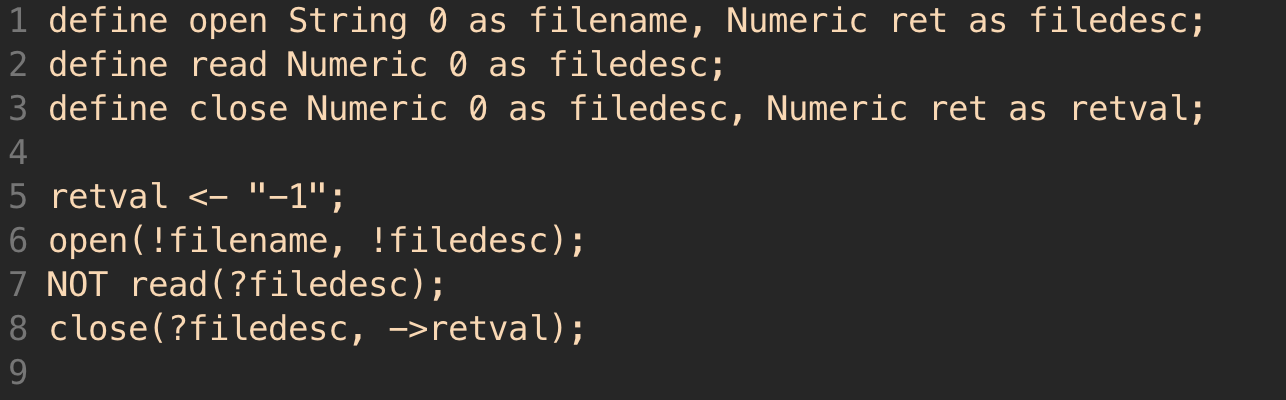
\includegraphics[scale=.50]{images/cslanglisting}
  \caption{A listing of a cslang program.  This program finds situations
  where a program opens a file and closes it without reading from it.  In
  such instances, it modifies the return value close call to be -1,
  indicating failure.}
  \label{fig:cslanglisting}
\end{figure}

\begin{figure}
  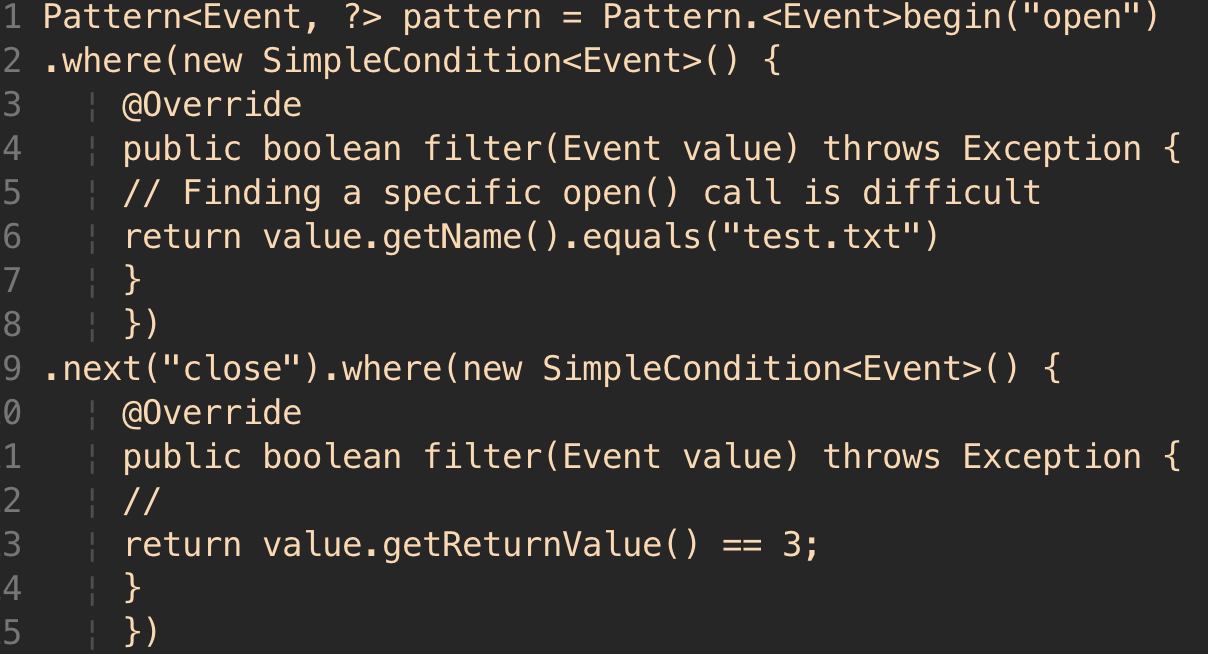
\includegraphics[scale=.50]{images/flinklisting}
  \caption{A listing of an Apache Flink program that does the same thing as the
  cslang program... I need to figure out what comparison stuff to put in
  this caption.}
  \label{fig:flinklisting}
\end{figure}


The decision to create a new programming language was not one we
undertook lightly,
as such an effort takes
a significant amount of work
to define,
implement, document, and support.
In this section we discuss the features we needed for this work
and why existing systems fell short.

First, we needed a language that treated state as a first-class citizen.
That is, it must allow the internal contents of events like argument data,
pointer addresses, and return values to be easily captured, manipulated, and
reused in subsequent operations.
This is necessary because,
at a very high level,
the purpose of system calls,
function calls,
rpc calls,
or other similar activity
is to allow an application
to gather data from an external module like a library or the operating
system.
As a result, it is frequently useful to be able to store the data returned by
one such action, modify it, and use it in matching actions.
For example, one may store the file descriptor returned by a {\tt
socket()} system call and use it later to match other related
communication system calls.
We found that this sort of usage was common across many types of
application activity further reinforcing our desire for a language that was
closely tailored to our needs on this in this area.

% Need to support new event stream formats easily?


\preston{We need to make sure we have given a best effort at shortening and
optimizing code from other languages with which we are making comparisons}

Our second requirement appears to be largely aesthetic at first glance
but there is a
larger purpose -- ease of learning and ease of use.  CSlang offers
improvements over existing languages along two primary fronts.
First, many event processing languages are verbose.
Consider figure~\ref{fig:cslanglisting}  which shows a
CSLang program that matches sequences where an application opens and closes
a file without reading from it.  When such a sequence is found, it is
modified such that the {\tt close()} call returns -1, indicating failure.
The main work of this program is performed in just four lines of CSlang
code.  For comparison, figure~\ref{fig:flinklisting} contains a Java program that
implements an approximation of the same program that was implemented in
CSlang~\ref{fig:cslanglisting}.
This program is only an approximation because it does not modify the return
value of the close() call as the CSLang program does.  Further, it assumes
that other work has been done to modify Apache Flink to enable the
consumption of a sequence of system calls.
In spite of these shortcomings, comparing the two programs remains
enlightening.  The Flink program is harder to read because it contains a
great deal of boilerplate code
that cannot be avoided due to its dependence on a fully-featured
programming language.  Other work that explores how developers read and
understand (or mis-understand!) code has shown that such constructs obscure
a programs meaning, harming understanding and
maintainability~\ref{CITEATOMSWORK}.
In light of this, we believe the benefits of a
new programming language
focused on allowing its users to get a lot of work done
with a small amount of easily-readable code are evident.

The second front involves CSlang's programming paradigm.
While other event processing languages tend toward functional or
declarative programming,
CSlang programs more closely follow an imperative programming style.
We came to this decision because studies
have shown that developers are more likely to be familiar and comfortable
with such a paradigm~\cite{XXXX}.  We believe this will make it easier for
developers to learn the language, foster greater popularity, and it aligns
with the goals presented in our motivating example.

Our final requirement is, perhaps, the most important.
We want CSlang programs to be capable of more than simply matching
a pattern of events and indicating that it has occurred.
Our review of the work on the SEA technique has shown that the ability to
{\textit modify} is central to forcing an application into situations where
it may fail rather than only passively monitoring for it to perform
problematic sequences.  While the feature-rich nature of several related
languages and libraries means it is likely possible to modify and output
incoming events, it is by no means a straightforward
and ergonomic experience.
Constructing CSlang to support output as a primary feature allows us to
easily describe the types of transformations needed to expose bugs.



\section{Language Overview}
\label{sec:Overview}

The PORT language allows its users
to completely describe a mutator
that can
accept a given event stream if it contains a particular
activity sequence. But, it can also produce a modified
output event stream
for application testing.
As noted in Section 2, standard
deterministic automatons or transducers can not accommodate these features.
Therefore, we instead compile a PORT program into
an  enhanced transducer that can operate over complex data structures.
The transducer consists of states, one of which is marked as the ``current state,'' and
a series of rules that govern when the current state should change based on the event type
and the parameters of an input stream element.
Additionally, these rules describe what modifications should be made to the input stream.

The rules cited above consist of logical comparisons between an event's parameter values, the values stored in the transducer's registers, or the literals specified directly in a program's code.
Using event processing techniques, PORT maps activity onto a
stream of \emph{events}, which can be defined here as individual interactions between the program and its environment, e.g.,
a single library, system, or remote procedure call.
Each event consists of a unique identifier (e.g. the name of the function being called) and a list of parameter values (e.g. the argument and return values of the called function).
Parameter values are drawn from a set of basic data values, such as strings and numbers, as well as user-definable record types.

PORT allows the user to ignore parameter values that are irrelevant for the particular task at hand.  It also can create a single abstract event from several that are semantically related, but have different event identifiers. The transducer description can then refer to just these abstract events rather than individually specify each event it contains.

A PORT transducer processes an input event stream as follows (illustrated in Figure~\ref{fig:Processing}).
Each item in an input
sequence is examined and the transducer's internal state is updated accordingly.
 Output is then produced based on the rules described in the transducer's program.
 In this way, 
 the transducer itself can be thought of as a finite sequence of \emph{actions}
 that may or may not be executed based on the values in the input stream. 
 The state of the transducer keeps track of the next action to be executed, as well as a valuation of a 
 finite number of \emph{registers} that hold data values.
 Whether or not an action is executed depends on a combination of the transducer state
 and the values of the current event.
 Therefore, executing an action consists of reading the next
event from the input stream, which may update some of the registers, and then writing the next event in the output stream.
%The parameter values in the output event may be computed from the (updated) registers.

\begin{figure}[t]
  \centering
  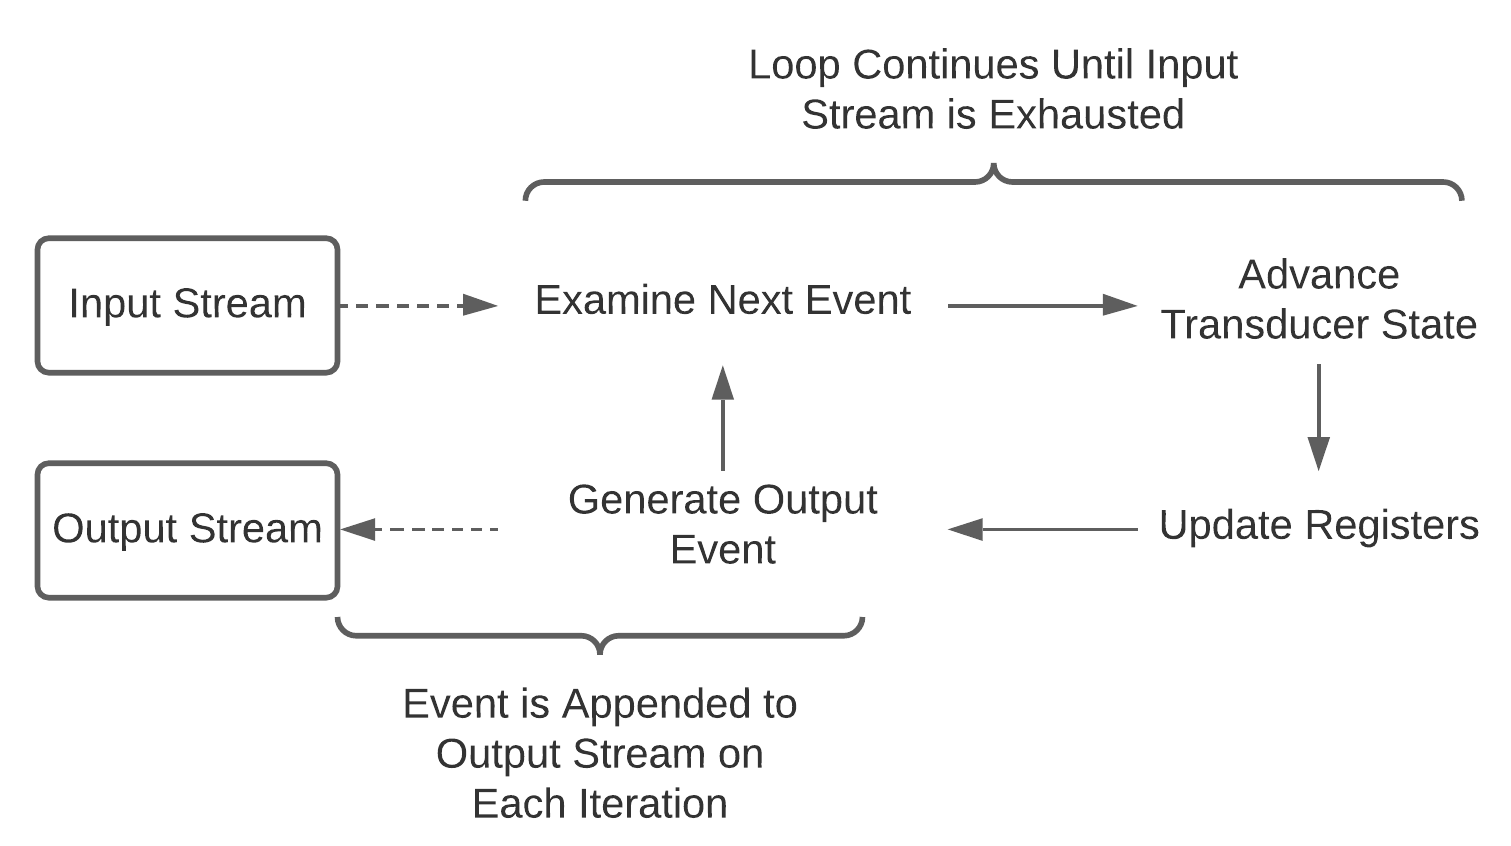
\includegraphics[scale=.6]{images/processing}
  \caption{A transducer individually processes each item in an input
  sequence, updating its internal state and producing output according
  to the rules described in its program.}
  \label{fig:Processing}
\end{figure}

%\iffalse
%Each action either processes a single event from the input stream, possibly additionally updating some registers of the transducer.
%
%This arrangement allows a user to find
%a specific category of events
%in a stream
%by matching a set of desired properties.
%To do so, the system specifies
%an identifier and a set of parameter value
%constraints.  For example, an unsuccessful {\tt close()} call could be
%found by looking for events with the identifier {\tt close} and a return
%value of -1.  This pairing of an identifier and a set of parameter
%constraints, referred to as an \emph{event pattern}, forms the primary mechanism in PORT for
%selecting specific events out of an activity stream.
%
%Implementing
%a program written in PORT 
%to identify a pattern of activity works as follows.
%As illustrated in Figure~\ref{fig:Processing}, a pattern is encoded as a list of datawords, and compared against
%events from the
%input event stream until the first dataword
%finds a ``match'' (matching is discussed further in
%Section~\ref{sub:PreambleAndBody}).  The event stream is next matched
%against the
%second dataword
%and so on until all datawords have been matched or the event stream is
%exhausted.
%
%
%%% talk about output.
%%Output is achieved through one further addition -- an output clause.  This
%%clause may be applied to any of the datawords in the list and describes
%%what output should be produced when the dataword it is associated with
%%matches an event.
%%
%%Datawords without an output clause are simply output without modification.
%%
%%In the following sections we discuss how these elements may be written as a
%%PORT program and transformed into a working mutator.
%
%
%\subsection{Preamble and Body}
%\label{sub:PreambleAndBody}
%
%\begin{figure}[h]
%\centering
%\begin{tabular}{c}
%\begin{lstlisting}
%########## Preamble ##########
%type statbuf {dev: String@0, stino: String@1};
%event fstat {fd: Number@0, st: statbuf@1};
%
%##########   Body   ##########
%finddev <- "st_dev=makedev(0, 4)";
%findino <- "st_ino=4026532069";
%out1 <- "foo";
%out2 <- "bar";
%fstat({st: {dev: ?finddev, stino: ?findino}});
%fstat({st: {dev: !finddev2, stino: !findino2}});
%fstat({st: {dev: ->out2, stino: ->out2}});
%\end{lstlisting}
%\end{tabular}
%\caption{An example PORT program with its preamble and body sections
%  labeled.}
%\label{lst:PreambleBody}
%\end{figure}
%
%
%
%A PORT program can be divided into two sections, the preamble and the body, as shown in
%Figure~\ref{lst:PreambleBody}. 
%The preamble defines the sorts of events
%expected
%to appear in an input event stream and the set of parameters
%under which future datawords will operate.  Specifying this information
%up-front configures a PORT mutator to
%automatically ignore extraneous information from the incoming stream.  This
%means that subsequent body statements only have to deal with events and
%parameters pertinent to the goal of the program.
%
%The body of a PORT program consists of a list of datawords that
%will configure the states and transitions
%of a mutator. 
%Each dataword (excluding usages of the NOT operator, discussed further
%in~\ref{subsub:NOT}) configures a single
%state and sets the rules that will govern how the mutator transitions into that state.
%Transitioning  into a new state is dependent on whether
%the current event``matches'' the requirements of the destination state.
%In PORT, a match requires satisfying three rules:
%
%\begin{itemize}
%\item{The event's identifier must match the destination state's identifier}
%\item{All parameters with the match operator applied must have a value equal to
%  the value currently stored in the associated register (discussed further
%    in Section~\ref{sub:DatawordOperators})}
%\item{All predicates must be satisfied by the parameter values in the
%  current event}
%\end{itemize}
%
%\fi


\subsection{Syntax and Semantics}
\label{sub:SyntaxAndSemantics}

Figure~\ref{lst:SyntaxGrammar} shows the grammar of PORT's core language.
A program is split into two parts: the \emph{preamble} consisting of type and event definitions, and the \emph{body} of the program which consists of a sequence of actions. 

\begin{figure}[t]
\centering
\begin{align*}
\mathit{program} ::= {} &  (\mathit{typedef} \mid \mathit{eventdef})^* \; \mathit{action}^*\\
\mathit{typedef} ::= {} & \mathtt{type}\; \mathit{id} \texttt{\{}\mathit{id} \texttt{:}\, t\, \texttt{@}\, n \; (\texttt{,} \mathit{id}\texttt{:} t\,\texttt{@}\,n)^*\texttt{\};}\\
\mathit{eventdef} ::= {} & \mathtt{event}\; \mathit{id} \; \mathit{variant} \; (\texttt{|}\; \mathit{variant})^*\texttt{;}\\
\mathit{variant} ::= {} & \texttt{\{}\mathit{id}\; \mathit{id}\texttt{:}\, t\,\texttt{@}\,n \; (\texttt{,} \mathit{id}\texttt{:}\, t\,\texttt{@}\,n)^*\texttt{\}}\\
%\mathit{body} ::= {} & \mathit{action}^*\\
%\mathit{action} ::= {} & \mathit{assignment} \mid \mathit{event}\\
%\mathit{assignment} ::= {} & \mathit{regid} \texttt{ <- } e\\
\mathit{action} ::= {} & \mathit{pattern} \texttt{ -> } \mathit{id}\,(e) \texttt{;} \mid \mathtt{not} \; \mathit{pattern} \texttt{;}\\
\mathit{pattern} ::= {} & \mathit{id}\,(p) \;\mathtt{with}\; b\\
p \in \mathsf{pexp} ::= {} & \texttt{\{} \mathit{id}\texttt{:}\, p \; (\texttt{,} \mathit{id}\texttt{:}\, p)^*\texttt{\}} \mid \mathit{regid} \mid c \\
e \in \mathsf{vexp} ::= {} & \mathit{regid} \mid c \mid e \,\texttt{+}\, e \mid e \,\texttt{-}\, e \mid \dots\\
b \in \mathsf{bexp} ::= {} & \mathtt{true} \mid \mathtt{false} \mid e == e \mid \ldots \mid p \;\mathtt{and}\; p \mid \dots\\
t \in \mathsf{texp} ::= {} & \mathtt{String} \mid \mathtt{Number} \mid \mathit{id} \mid \dots
\end{align*}
\caption{Grammar of PORT's core language.}
\label{lst:SyntaxGrammar}
\end{figure}

\paragraph*{Preamble}

The abstract event consists of a name and a record of named fields that hold data values of interest. As an example, consider the event definition:
\begin{lstlisting}[numbers=none,xleftmargin=0em,gobble=2,columns=strict]
  event rd {read fdesc: Number@0} | {recv fdesc: Number@0};
\end{lstlisting}
This definition maps the concrete events named \lstinline+read+ and \lstinline+recv+ to the abstract event \lstinline+rd+. The parameter values of the concrete events are abstracted to a record consisting of a single field \lstinline+fdesc+ that holds a value of type \lstinline+Number+. The notation \lstinline+fdesc: Number@0+ in each variant indicates that the value of \lstinline+fdesc+ is the 0th parameter of the corresponding concrete event. Note that all variants must map their parameters to the same record type.

If an event definition defines an abstract event in terms of a single variant for which the concrete event name coincides with the name of the abstract event, then the former can be omitted in the variant.

Event definitions have three distinct functions. First, they allow a PORT program to ignore
irrelevant parameter values in concrete events. Second, they can map semantically-related concrete events to the same abstract event, and lastly it permits any modifications of record fields to be mapped back to corresponding modifications of the underlying concrete events.
%These operations can be accomplished even if the values tracked by the
%abstract event occur at different positions in the parameter lists of the concrete events.

The abstraction mechanism used for the parameter lists of concrete events can also be applied to the values themselves. For instance, the 1st parameter of an \lstinline+fstat+ system call is a status buffer that consists of a list of values. \emph{Type definitions} can be used to abstract such compound values into records. The following PORT code defines an abstract \lstinline+fstat+ event that tracks only the device identifier, inode number, and mode of the status buffer:
\begin{lstlisting}[numbers=none,xleftmargin=0em,gobble=2]
  type SB {dev: String@0, ino: String@1, mode: String@2};
  event fstat {fdesc: Number@0, sbuf: SB@1};
\end{lstlisting}

%\iffalse
%Each statement specifies an event ``variety'' and a list of
%parameters that should be accessible in later dataword statements.
%An event's variety will correspond
%with the system call name, RPC call name, or, in the case of other activity
%representations, a unique identifier that allows events of the same
%variety to be picked out of a stream.
%
%A variant definition allows several event definitions to be combined under
%a single identifier.  This identifier may then be used in a dataword
%statement to match any of the collected events.
%
%  This feature arose as a
%result of situations where one of several system calls could be used to
%perform the same operation (e.g. {\tt read()} and {\tt recv()}).  The
%concrete syntax necessary to achieve this pairing is shown in the example
%above where the variant ``bothread'' is defined such that it will match
%either a {\tt read()} or {\tt recv()} system call.
%\fi



\paragraph*{Body}
The actions in the body of a PORT program describe how the input event stream is transformed to the output event stream. An individual input event is matched and transformed by an action of the form
\[\mathit{id}_1(p) \;\mathtt{with}\; b \texttt{ -> } \mathit{id}_2\,(e)\texttt{;}\]
This action matches the next (abstract) input event against the \emph{pattern} $\mathit{id}_1(p)$ subject to the constraint $b$. The action is triggered if the name of the matched event is $\mathit{id}_1$ and its record satisfies the constraints imposed by $p$ and $b$. The semantics of pattern matching is similar to the way  expressions are pattern matched in functional programming languages. In particular, a variable occurring in a pattern refers to a register of the transducer. If the pattern matches the event, then the register is assigned to the corresponding value. For example, consider the pattern:
\begin{lstlisting}[numbers=none,xleftmargin=0em,gobble=2]
  fstat({fdesc: fd2, sbuf: {dev:rdev, stino: rino2}})
\end{lstlisting}
When matched against the event
\begin{lstlisting}[numbers=none,xleftmargin=0em,gobble=2]
  fstat({fdesc: 4, sbuf: {dev:"st_dev=makedev(0, 4)",
                             ino: 42, mode="S_IFCHR|0666"}})
\end{lstlisting}
the match would succeed and assign the value \lstinline+4+ to register \lstinline+fd2+, \lstinline+"st_dev=makedev(0, 4)"+ to register \lstinline+rdev+, and \lstinline+"S_IFCHR|0666"+ to register \lstinline+rino2+.

The Boolean expression $b$ is evaluated after the initial match of $\mathit{id}_1(p)$ succeeds. If $b$ evaluates to \lstinline+true+ then the action takes effect. Otherwise, the match fails and the registers are reset to their original values before $\mathit{id}_1(p)$ was matched.

When an action takes effect, the matched input event is consumed and an output event is appended to the output stream. This output event is described by $\mathit{id}_2\,(e)$ in the \emph{output clause} of the action. If $\mathit{id}_2=\mathit{id}_1$, then $e$ can be a \emph{partial} record expression, describing only those parts of the input record that should be modified by the action. Record fields that are not specified by $e$ are copied from the input event to the output event. If the record types of the input and output events differ, $e$ must describe the output record completely.

For example, consider the action:
\begin{lstlisting}[numbers=none,xleftmargin=0em,gobble=2]
  fstat({fdesc: rfd2, sbuf: {dev:rdev, ino: rino2}})
    with rfd2 == rfd and rdev == "st_dev=makedev(0, 4)"
    -> fstat({sbuf:{ino: rino}});
\end{lstlisting}
This action matches the \lstinline+fstat+ event given above, assuming the register \lstinline+rfd+ has value \lstinline+4+ before the match. Moreover, if the register \lstinline+rino+ has value \lstinline+43+ before the action is executed, then the action produces the output event:
\begin{lstlisting}[numbers=none,xleftmargin=0em,gobble=2]
  fstat({fdesc: 4, sbuf: {dev:"st_dev=makedev(0, 4)",
                             ino: 43, mode="S_IFCHR|0666"}})
\end{lstlisting}

For convenience, we have included a syntactic short-hand that allows one to more compactly express common kinds of patterns. First, one often needs to express that the value of a matched record field is equal to the current value of a register. In the action above, the field \lstinline+fdesc+ of the matched \lstinline+fstat+ event must be equal to \lstinline+rfd+ for the match to succeed. This constraint can be expressed more succinctly by replacing \lstinline+rfd2+ with \lstinline+?rfd+ in the pattern of the action. Doing so ensures that the matched value is equal to \lstinline+rfd+ without changing the value of \lstinline+rfd+. The equality \lstinline+rsd2 == rsd+ can then be omitted from the \lstinline+with+ clause.

Next, the \lstinline+with+ clause can also be omitted altogether from an action, in which case $b$ defaults to \lstinline+true+. Likewise, the output clause can be omitted and the matched input event can simply be copied to the output stream. Finally, an action is replacing only the value of a field, and the action is not dependent on the old value, then the modified field value can be specified directly in the pattern using the notation \lstinline+->$e$+. Here, the expression $e$ determines the new value to be stored in the field.

Using this syntactic short-hand, the action given above can be expressed more compactly as:
\begin{lstlisting}[numbers=none,xleftmargin=0em,gobble=2]
  fstat({fdesc: ?rfd, sbuf: {dev:"st_dev=makedev(0, 4)", ino: ->rino}});
\end{lstlisting}


\paragraph*{Implicit repetition and negated patterns}
%In our design of PORT we have decided against the inclusion of the repetition and choice constructs supported by general-purpose stream processing languages. This design decision greatly simplifies the transducer construction as we do not have to deal with elimination of epsilon transitions expressing nondeterministic choice. 

PORT simplifies the handling of an unbounded input stream by using implicit repetition semantics.
Any event in the input stream not matched by the current action is simply copied to the output stream. The transducer moves on by attempting to match the next input event against the current action.

Sometimes, it is necessary to constrain this implicit repetition mechanism by disallowing the appearance of certain events in the input stream before an event  matched by the current action is encountered.  This can be done by \emph{negated patterns}, which take the form \lstinline+not id$(p)$ with $b$+. If an event that matches the pattern \lstinline+id$(p)$ with $b$+ is encountered before the next positive action in the program takes effect, then the transducer aborts. For instance, the program in Fig.~\ref{fig:PORTListing} uses a negated pattern to ensure that no \lstinline+read+ system call is executed on the opened file with file descriptor \lstinline+fd+ before the file is closed.

\paragraph{Explicit Repetition}
PORT also supports matching clearly defined sequences of events.  This functionality is useful when a desired pattern
contains some unknown number of repetitions of one or more events.
This functionality behaves similarly to a Kleene star as provided by many regular expressions engines.
That is, the generated transducer accepts zero or more repetitions of the specified sequence of events.
Output is only produced if a complete repetition of sequence is encountered.
All previously discussed functionality and behavior holds true for the sequence being repeated.

%\iffalse
%This production triggers the creation of a mutator with only a starting
%state.  This state is accepting in two situations:
%\begin{itemize}
%  \item{When no other states are added to the automaton by subsequent
%    statements}
%  \item{When the only other states added to the automaton are NOT states
%    which reject sequences they match}
%\end{itemize}
%In all other cases this is a rejecting state that produces no output.
%
%
%\begin{quote}
%\centering
%\textbf{assignment: x <- e}
%\end{quote}
%
%Assignment statements store the value of an expression, e, into a named
%register on the mutator being described.
%If the register does not exist,
%it is created;
%otherwise its stored value is overwritten.
%Registers may contain Number or String values.  Register contents
%may be used in subsequent statements to specify parameter values that must
%be present in order for an event to match, or as values to be output.
%
%
%
%\begin{quote}
%\centering
%\textbf{dataword: id paramexp predexp outputexp}
%\end{quote}
%
%
%Dataword statements are responsible for adding new states to the
%mutator.  This means they must specify any register operations,
%transition conditions, and output associated with these new states.  To
%tackle this complexity we will address each part of this production
%individually.
%
%\textit{id paramexp}
%
%The parameter expression offers an opportunity to examine and store
%parameter values from the current event.  PORT supports two operators
%that may be applied to parameter expression members.  The match operator
%(!) allows for the rejection of otherwise matching events
%by enforcing a required value on a
%chosen parameter while the store operator (?) copies a value from the
%current event and stores it in the specified register.
%
%
%\textit{predexp}
%
%Predicate expressions are used to place additional restrictions that must
%be met if the mutator is to advance into the newly created state.  These
%restrictions compare values from the current event to either register
%values or literal values.
%
%\textit{outputexp}
%
%An output clause controls the output that will be produced when its
%associated state is entered.  The nature of this output is controlled by a
%parameter expression that specifies which parameters of the current event
%should be replaced with a value from a register.  If a parameter is not
%included in the parameter expression, its original value is used.
%Similarly,
%if an output clause is omitted, the output will be the
%original, unmodified event.
%
%\subsection{Dataword Operators}
%\label{sub:DatawordOperators}
%
%PORT supports two operators that may be applied to a dataword's
%parameters: Match and Store.  These operators are central components in
%the description of a mutator.  Each operator is associated with a dataword
%parameter and a register or literal value.
%
%\subsubsection{Store Operator (!)}
%
%The store operator, ``\textit{!}'', adds a requirement that the
%mutator should extract a parameter value from the current event and store
%it in the specified register.  These values may then be modified by
%register expressions, combined with the match operator to add more
%entry requirements to a state, or used in output expressions.
%
%\subsubsection{Match Operator (?)}
%
%The match operator, ``\textit{?}'',
%allows PORT's user
%to provide additional conditions
%that an event's parameter values must meet
%in order to match a dataword.
%Specifically,
%the operator requires
%that its parameter value equal the
%register value
%or literal value
%to which it is applied.
%This functionality is
%useful when a value is stored upon the occurrence of one event
%and then used to identify an associated event expected to appear later.
%A common example of this pattern is storing the file descriptor
%returned by an {\tt open()} or {\tt socket()} call into a register
%and using it to find related {\tt read()} further along in a system call
%trace.
%
%\subsubsection{The NOT keyword}
%\label{subsub:NOT}
%
%The NOT keyword is used to reject a sequence if the event being
%described is encountered.  This is done by creating a ``trap''
%rejecting state.  Such a state follows the same entry rules
%as a normal state but has no outgoing transitions.  This guarantees that a
%recording containing matching events will be rejected.
%We found this capability useful for writing programs that could identify
%situations where an application incorrectly performs one or more steps of a
%complex operation.
%
%
%
%\fi
%
%%%%% We need to talk about how we are different from other
%%%%% languages that are regular-expression like here
%%\subsection{Inspiration from Regular Expressions}
%
%%%% Local Variables:
%%%% mode: latex
%%%% TeX-master: "paper"
%%%% End:
%
\section{Architecture and Implementation}

The implementation of PORT consists of several related
components that allow a program to be used to analyze a stream of
application activity.
In this section we discuss the most important of these components and some
of the decisions that went into their design and operation.
PORT is available for use at: \textit{Link Removed for Blinding Purposes}.
\label{SEC:architecture}

\begin{figure}
  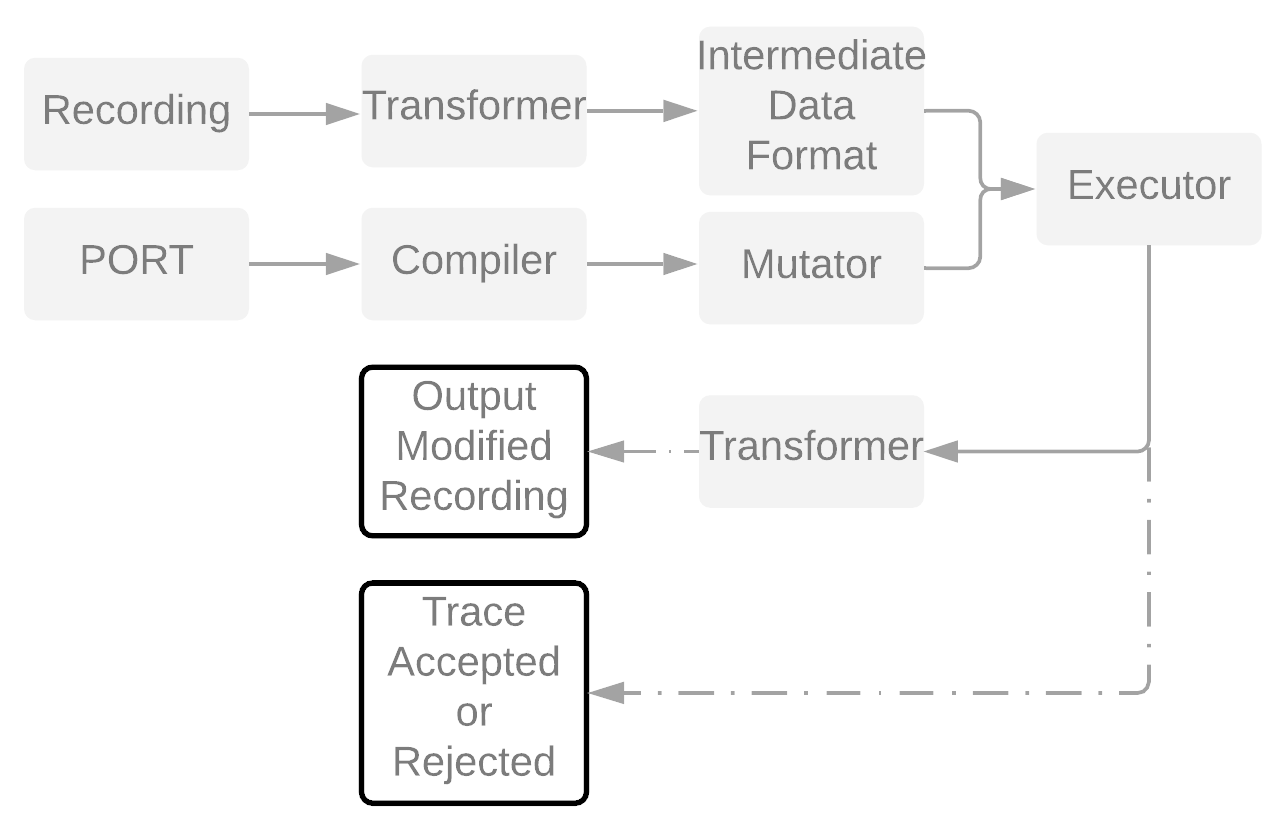
\includegraphics[scale=.19]{images/architecture}
  \caption{Overview of PORT compiler and run-time components.}
  % \caption{The PORT compiler produces a mutator that operates over a
  % generic intermediate data format that contains the contents of an application
  % recording.  This is facilitated by an executor program provides each
  % event in the input stream to the mutator in turn.  The mutator updates
  % its own internal state based on the contents of each event and, if
  % appropriate, produces a modified output event.  At the end of processing,
  % the mutator either accepts or rejects the input stream based on whether
  % or not its pattern was found.}
  \label{fig:architecture}
\end{figure}

\subsection{The PORT Compiler}

The PORT compiler is responsible for constructing a transducer
from a PORT program.
%PORT is a compiled rather than an interpreted language because
%the earlier SEA work showed that this sort of program is typically
%compiled a few times during construction
%and executed many times over many different applications.
%By compiling ahead of time we save the performance cost associated with other
%approaches like just-in-time compilation or execution via an interpreter.
Compilation happens in two phases.  In the first phase, the program text is
parsed into an abstract syntax tree using an LALR parser.
In the second, the
contents of the AST are used to construct the transducer.
This transducer is then serialized to
disk so that it may be stored and reused.

\subsection{The Internal Data Format}

We wanted to make PORT flexible so the SEA technique
could
work with many different sorts of
activity representations beyond system calls.
Such flexibility would both prevent PORT from being tied to specific recording formats or activity representations and simplify the process of modifying parameter in a format-agnostic fashion.
This required a method to cleanly separate the details of how
an application's event activity is recorded from the representation of this event stream that is
processed by a transducer.
Our solution is twofold.  First, we develop an intermediate data format
(IDF) that
stores the key components, such as parameter and return values,
for application activities like function
and system calls.  This format supports primitive string and numeric
values as well as arbitrarily nested structures in the form of records.
The language and compiler currently do not support unbounded arrays. However, extending PORT with arrays is relatively straightforward.

% The decision to include these features
% was based on the Linux kernel's system call implementation
% which allows system call inputs and outputs in the form of primitive data
% values and complex structures. These capabilities would be necessary
% if PORT was going to support system calls.

The actual activity stream of an application is converted from its original representation into IDF and
back using a \emph{transformer} module. The transformer parses each activity entry,
extracting the relevant data, and assembles this information into an IDF
event record.  These event records comprise the input stream of the transducer.
The output event stream is then converted by the same transformer module
back into the original activity representation. We have implemented transformers for different kinds of activity streams including system call and RPC call sequences.

\subsection{Executing a PORT Program}

The ``Executor'' module implements the PORT run-time environment.
% Unlike an executable program, a compiled PORT program is a static entity
% that cannot run by itself.  Instead, a component we refer to as the
% ``PORT Executor'' is responsible for carrying out the ancillary work
% required to analyze an application recording with a mutator.
The tasks performed by this module include deserializing a stored mutator from disk,
converting the selected input stream to IDF,
running the transducer,
using the appropriate transformer to translate the output stream back to the original activity representation, and reporting whether the input sequence was
accepted or rejected by the transducer.

%%% Local Variables:
%%% mode: latex
%%% TeX-master: "paper"
%%% End:

\section{Evaluation}
\label{SEC:evaluation}

With our prototype in hand we organized a set of
evaluations that would let us know if the CSlang would be effective
in real world situations.
We designed our tests to answer the following questions:

\begin{itemize}

    % Re-implementing CS anomalies
  \item{Can CSlang express the sorts of anomalies used by SEA to identify
    bugs?}

    % Extending to support RPC formats
  \item{How easy is it to extend CSlang to support activity representations
    other than system calls?}

    % Dornhackl et al. defining maliciousness
  \item{What sorts of problems can be addressed by employing CSlang on
  non-system-call activity representations?}

    % Performance information
  \item{Can CSlang process input streams in a reasonable amount of time?}

\end{itemize}


\subsection{Expressing SEA Anomalies}
\label{sub:SEAAnomalies}
Given that this work was motivated
in large part
by the effectiveness of the SEA technique,
our first test of CSlang was using it to reproduce the anomalies described
in the original paper.
We wanted to ensure that
the language we developed
would be sufficiently powerful
to describe the anomalies the
SEA research team used to
find bugs.
Specifically,
we set out to test CSlang's ability to recreate
the study's Unusual Filetype mutator,
and its Cross-disk file move checkers, which were used to identify
the bulk of
the bugs that were found.
Our hope was that by using CSlang we could eliminate boiler plate code,
save effort by handling common tasks automatically, and improve reliability
by providing a structured way to modify and output system call sequences.

\begin{figure}[H]
\centering
\begin{tabular}{c}
\begin{lstlisting}
event statbuf {mode: String@2};
event anystat {stat sb: statbuf@1}
           | {lstat sb: statbuf@1}
           | {fstat sb: statbuf@1};
newmode <- "st\_mode=S\_IFBLK";
stat({}) -> stat({sb: {mode: ->newmode}});
\end{lstlisting}
\end{tabular}
\caption{This program identifies a stat, lstat, or fstat call and modifies
  the ST\_MODE member of its statbuf output parameter to contain the value
  "S\_IFBLK."  This indicates that the file being examined is a block device
  rather than a regular file.  The value used in modifying ST\_MODE is
  controlled by changing the value stored in the newmode register.}
\label{lst:UnusualFiletypeCSlang}
\end{figure}

\subsubsection{Creating the Unusual Filetype Mutator}
\label{subsub:UnusualFiletype}
For the first phase of this work,
we used CSlang to implement an ``Unusual Filetype''
mutator.
This mutator, presented in
Figure~\ref{lst:UnusualFiletypeCSlang},
should take an input trace
that contains a call to either {\tt stat()},
{\tt fstat()},
or {\tt lstat()}
and modify the call's result data structure such
that its {\tt ST\_MODE} member will contain a value
that indicates an unusual filetype.
Table~\ref{tbl:ST_MODEValues}.  As can be seen in
Figure~\ref{lst:UnusualFiletypeCSlang}, CSlang's semantics mean such an
operation can be captured with only a handful of lines of code.  In the
figure
lines 1 through 4 define what {\tt stat()}, {\tt fstat()}, and {\tt
lstat()} calls look like and which parameter contains the result buffer.
Line 6 generates an accepting state that, when entered, produces an output
system call with a modified value in the return structure's {\tt st\_mode}
field.  Such output can then be used to modify the results of a running
application's system calls in order to carry out the remaining steps of the
SEA technique.

CSlang's advantages are made even more obvious when the CSlang Unusual
Filetype mutator is compared to a program that implements the same
functionality in a general purpose programming language like Python.
Figure~\ref{lst:UnusualFiletypePython} shows an excerpt from a 55 line
Python program taken from the SEA paper's CrashSimulator that performs the
same mutation described above.  Comparing this listing to
Figure~\ref{lst:UnusualFiletypeCSlang} shows several key differences:

\textit{Minimal boilerplate code:} The CSlang program lacks the boilerplate
code associated with
reading an input trace, managing mutator state, and producing output.
This is possible because CSlang's capabilities are narrowly defined to
only describe the states and operations of a mutator.  This means these
functions can be generically implemented within CSlang's core eliminating
the need for users to do so manually.

\textit{No code required to filter out uninteresting calls:}
CSlang's user does
not need to write any code to exclude system
calls outside of the desired set.  Each statement defines a new state with
incoming and outgoing transitions configured such that any system calls not
dealt with in the CSlang program are ignored.

\textit{Easy to modify call contents:}  CSlang's operators make it
trivial to change components of a system call
and produce output without having to regenerate the remainder of its
parameters.
This is a far cry
from the Python program which relies on manual, fragile string manipulation
to achieve the same effect.


\begin{figure}[H]
\centering
\begin{tabular}{c}
\begin{lstlisting}
... 3 lines omitted ...
class UnusualFiletypeMutator(GenericMutator):
  def \_\_init\_\_(self, filetype='S\_IFREG', name=None, file\_descriptor=None):
  ... 6 lines omitted ...

  def mutate\_syscalls(self, syscalls):
    index = self.\_find\_index(syscalls)
    for i in range(len(syscalls[index].args)):
      if 'st\_mode' in str(syscalls[index].args[i].value):
        syscalls[index].args[i].value=re.sub(r'S\_IF(\w*)', self.filetype, syscalls[index].args[i].value)

... 13 lines omitted ...

  def identify\_lines(self, tm, que, thread\_condition):
    while True:
      ... 3 lines omitted ...
      if syscall\_trace['syscall'].name.startswith('fstat'):
        if self.file\_descriptor:
          if self.file\_descriptor != syscall\_trace.args[0].value:
            continue
        self.opportunity\_identified(syscall\_trace, self.mutator\_name, que)
      if syscall\_trace['syscall'].name.startswith('stat') or syscall\_trace['syscall'].name.startswith('lstat'):
        if self.name:
          if self.name != syscall\_trace.args[0].value:
            continue
        self.opportunity\_identified(syscall\_trace, self.mutator\_name, que)
\end{lstlisting}
\end{tabular}
\caption{This is a Python module taken from SEA's CrashSimulator that
  implements the ``Unusual Filetype'' anomaly.  This listing has been
  shortened by removing CrashSimulator specific-code so that a fair
  comparison can be drawn between it and the same mutator implemented in
  CSlang.}
\label{lst:UnusualFiletypePython}
\end{figure}

\subsubsection{Creating the Cross-Disk Move Checkers}

The second phase of this work involved the recreation of a set of
``checkers'' that could examine an application as it moved a file from one
disk to another and report whether or not the operation was carried
out correctly.  These checkers took advantage of the fact that the Linux
{\tt rename()} system call does not support moving files from one disk to
another.  This means applications have to perform this complex
operation manually.  Earlier work on the SEA technique
identified XX steps required to
correctly perform such a move by examining the source code of the ``mv''
command.  With this knowledge, they
implemented a set of checkers to identify situations where one
or more of these steps were not carried out correctly.
When applied to real world applications,
these checkers were able to identify bugs
in many popular applications and libraries that offered file movement
capabilities.

Similar to the Unusual Filetype described in
Section~\ref{subsub:UnusualFiletype},
we first implemented the
set of checkers in CSlang.  Figure~\ref{lst:Cross-DiskMoveCSlang} shows one
such checker that ensures {\tt fstat} is used after a file is opened but
before it is moved.  This pattern indicates that an application may be
storing the {\tt inode} number of the file -- a step necessary to prevent a race
condition where the file is replaced during the move process.  When
we compare this checker to the Python version in
Figure~\ref{lst:Cross-DiskMovePython} many of the qualities we discussed
above are apparent.  The CSlang version is more concise and its meaning is
less obscured by boilerplate and state management code that makes up the
bulk of the Python version.

This exercise did expose one of CSlang's shortcomings.
The Python checker in Figure~\ref{lst:XattrsPython},
which ensures an application
preserves all of a file's extended attributes and re-applies them the
destination file after the move.
The difficulty creting this checker
in CSlang was due to two factors.
First, CSlang does not support looping with a
runtime-defined number of iterations.  This is necessary to capture all
calls to {\tt getxattr()}.
Further, CSlang does not support a list data structure to store the values
retrieved by such calls and ensure they have all been applied with a
corresponding call to {\tt setxattr()}.
We are evaluating these deficiencies and plan to address them in the
future.

\begin{figure}[H]
\centering
\begin{tabular}{c}
\begin{lstlisting}
\\ This is absolutely a fake listing that will be changed out for a real
\\ one!!  Preston -> Don't forget to do this!
#include "stdio.h"

int main() {
    printf("Hello world!\n");
    return 0;
};
\end{lstlisting}
\end{tabular}
\caption{One of the cross disk move checkers implemented in CSlang}
\label{lst:Cross-DiskMoveCSlang}
\end{figure}


\begin{figure}[H]
\centering
\begin{tabular}{c}
\begin{lstlisting}
\\ This is absolutely a fake listing that will be changed out for a real
\\ one!!  Preston -> Don't forget to do this!
#include "stdio.h"

int main() {
    printf("Hello world!\n");
    return 0;
};
\end{lstlisting}
\end{tabular}
\caption{One of the cross disk move checkers implemented in Python}
\label{lst:Cross-DiskMovePython}
\end{figure}

\subsection{Extending CSlang}

While the above results are encouraging, we wanted to ensure that CSlang's
usefulness was not limited to system call manipulation.
A logical next step would be to test CSlang's capabilities when working
with a higher level, but similarly structured, activity representation.
After some consideration we settled on JSONRPC and XMLRPC.  These formats
were ideal because they are well defined, popular, and both have well
supported parsing libraries or modules.

To evaluate CSlang's ability to work with these representations we
constructed transformer modules that could convert these formats into our
intermediate data format.
We tested our implementation by writing CSlang programs that could modify
activity streams similar to the examples presented in the JSONRPC
2.0~\cite{jsonspec} and XMLRPC~\cite{xmlspec}
specifications.  One such program is shown in
listing~\ref{lst:JSONProgram}.  This program matches a pattern of ``test''
and ``update'' calls and, if the pattern is found, the final update call's
parameters are replaced with the contents of two registers.

JSONRPC support required handful of hours of effort and XMLRPC
support, whose implementation we precisely timed, was completed in three
hours and thirty-two minutes.  Based on the ease and speed with which we
ere able to complete these additions we are confident that CSlang can be
quickly adapted to support new activity representations as required.

\begin{figure}[H]
\centering
\begin{tabular}{c}
\begin{lstlisting}
event update {up1: Numeric@0, up2: Numeric@1};
event test {tp1: Numeric@0, tp2: String@1};
num <- 45;
str <- "alpha";
update({up1: !pone, up2: !ptwo});
outone <- 999;
outtwo <- 888;
test({tp1: ?num, tp2: ?str});
update({up1: ->outone, up2: ->outtwo});
\end{lstlisting}
\end{tabular}
\caption{This CSlang program matches a pattern of JSONRPC calls to
  ``update'' and ``test.''  If the pattern is identified, the final call to
  update is modified so that its first two parameter values are replaced
  with the values stored in the outone and outtwo registers.}
\label{lst:JSONProgram}
\end{figure}


\subsection{Utilizing CSlang's Flexibility}
In addition to novel formats, we wanted to see if CSlang could be used to
represent proven-useful models from other work.  One candidate for this
effort is the work on describing malicious behavior done by Dornhackl et
al. in 2014~\cite{Dornhackl2014}.  This work improves upon static malicious
behavior detection using signatures by creating formal models that can
detect misbehavior in an application's dynamic activity.  This is done
using two models: one that describes malicious activity in the form of a
series of tasks and a second that maps these tasks onto the concrete
Windows API calls required to carry out these tasks.

CSlang is particularly well suited to implementing the second model.  This
requires a mechanism for first grouping a set of similar API calls
into a single operation and then describing a malicious task in terms of
these aggregate operations.  CSlang supports the former using variants.
For example, the work proposes grouping the API calls that may be used to
open a Windows registry key as is shown in Figure~\ref{lst:DornhacklOpen}.

\begin{figure}[H]
\centering
\begin{tabular}{c}
\begin{lstlisting}
OPEN => RegOpenKeyA NtOpenKey
  | RegOpenKeyW NtOpenKey
  | RegOpenKeyExA NtOpenKey
  | RegOpenKeyExW NtOpenKey
\end{lstlisting}
\end{tabular}
\caption{Grouping of Windows API calls for opening or creating a Windows
  registry key into an OPEN operation as per Dornhackl et al.}
\label{lst:DornhacklOpen}
\end{figure}


In the above grammar, each symbol beginning with ``Reg'' represents a user
API that opens or creates a registry key.  {\tt NtOpenKey} always follows
each of these calls because it is the underlying ``native'' call that
Windows makes to actually perform the operation.
The grouping and execution semantics for this operation can be expressed
in CSlang as shown in Figure~\ref{lst:CSlangOpenReg}.


\begin{figure}[H]
\centering
\begin{tabular}{c}
\begin{lstlisting}
 open {RegOpenKeyA ...}
    | {RegOpenKeyW ...}
    ... further varients omitted

  event NtOpenKey {...};

  open({...});
  NtOpenKey({...});
\end{lstlisting}
\end{tabular}
  \caption{Abstract CSlang program (with parameters
  omitted) that groups the Windows API calls responsible for opening or
  creating a Windows registry key into an open operation.  It also shows
  how the requirement that NtOpenKey follow any of these calls can be
  captured.}
\label{lst:CSlangOpenReg}
\end{figure}

Dornhackl et al. used this strategy to describe a pattern that, if
detected, would indicate
a Windows registry key was being installed
that would cause some malicious action
the next time the machine was restarted.  We can use CSlang to group the
Windows API calls into the same operations as the original work and
construct a program that could perform this detection (assuming CSlang were
extended to support Windows).  Such a program appears in
Figure~\ref{lst:CSlangRegDetect}.  This program groups API calls into OPEN,
SET, and CLOSE operations and searches for a pattern that
indicates
an application is
setting an autostart key.  The CSlang program is further able to express
that the pattern must appear for a specific registry key using the value
stored in the ``regkey'' register.

\begin{figure}[H]
\centering
\begin{tabular}{c}
\begin{lstlisting}
  variant open {RegOpenKeyA ...}
          |    {RegOpenKeyW ...}
     ... further variants omitted ...
  event NtOpenKey {...};
  variant set {RegSetValueExA ...}
          |   {RegSetValueExW ...}
     ... further variants omitted ...
  event NtSetValueKey {...};
  event close {RegCloseKey ...};
  event NtClose {...};

  open({...});
  NtOpenKey({...});
  set({...});
  NtSetValueKey({...});
  close({...});
  NtClose({...});
\end{lstlisting}
\end{tabular}
  \caption{This listing shows an abstract CSlang program (with parameters
  omitted) that detects situations where an application is maliciously
  installing an ``autostart'' Windows registry key.  It does so by
  implementing the pattern described by Dornhackl et al.  Unimportant
  parameters are omitted and the number of API calls in each group has been
  reduced in order to save space.}
\label{lst:CSlangRegDetect}
\end{figure}


\subsection{CSlang's Performance}

It doesn't matter how useful a tool may be
if it takes too long to complete its work.
Though our implementation is
only a prototype, we wanted to make sure that its performance was not
overly slow.
Our performance evaluation
is focused on the time required
to identify specific
patterns within real world system call traces.
We recorded test traces
from two popular network applications -
NCat,
and
Python's http.server.
These
were chosen because they are widely used and
offer increasing levels of complexity against which we can evaluate
CSlang's effectiveness.

Our test operated as follows.  The applications were configured to service
a simple piece of content (a single string in the case of NCat) and were
recorded using {\tt strace} while handling a request from a remote client.
The strace
recordings\footnote{Recordings were pre-processed to remove system calls
related to executable loading and process creation} were then processed using the CSlang program from
Figure~\ref{lst:RealWorldPerformance},  which
identified the sequence of system calls that implement
a server's request handling
loop.  Table~\ref{tbl:RealWorldPerformance}
shows the times in seconds required to perform this identification on each
web server as well as the total number of system calls in each trace.

\begin{figure}
  \begin{tabular}{|c|c|c}
                & Time in Sec. & Num. Syscalls.\\
              \hline
  http.server   & 0.104 Sec.   & 297   \\
  NCat          & 0.092 Sec.   & 43      \\
\end{tabular}
\caption{Time in seconds to process the listed number of events of each format.}
\label{tbl:RealWorldPerformance}
\end{figure}

\begin{figure}[H]
\centering
\begin{tabular}{c}
\begin{lstlisting}
event accept { accept fd: Numeric@ret} | { accept4 fd: Numeric@ret};
event anyrecv { recvfrom fd: Numeric@0} |
  { read fd: Numeric@0} |
  { recv fd: Numeric@0};

event anysend {sendto fd: Numeric@0}
  | { write fd: Numeric@0}
  | { send fd: Numeric@0};

event close {fd: Numeric@0};

accept({fd: !storefd});
anyrecv({fd: ?storefd});
anysend({fd: ?storefd});
close({fd: ?storefd});
\end{lstlisting}
\end{tabular}
\caption{This CSlang program matches patterns where a server application
  accepts a connection, receives a request, sends a response, and closes
  the connection.  The program uses variants to handle cases where
  applications use different system calls to perform some common action
  (e.g. receiving data from a socket)}
\label{lst:RealWorldPerformance}
\end{figure}

The results in Table~\ref{tbl:RealWorldPerformance} show that, as expected,
CSlang's
processing time increases in line with the total number of system calls
present in a recording.  We anticipate that much of this processing cost is
associated with setting up a Python execution environment and that a more
optimized implementation could improve performance gains in this area.
Further,
it is likely that CSlang's performance is closely tied to
disk throughput,
and that advancing the mutator
as each system call is evaluated
adds little additional overhead.
A condition with varying disk
speeds could be designed to confirm this suspicion.  As a whole, our
results indicate that CSlang's performance is not a limiting factor to its
usage in real-world situations.

\section{Related Work}
\label{SEC:related-work}

One of the ultimate goals of developing PORT
was to make it easier for developers to
create tools capable of detecting intrusion,
performing fault injection,
or conducting other program-level testing.
To design such a language,
we consulted
previous work
in processing sequences of events, such as
system calls, RPC invocations or
web-browser events.
Below, we discuss some of the more significant work in these areas.

\paragraph{System Call Stream Processing Applications.}

System call based intrusion detection systems fall into two types: misuse and anomaly detection.
The former search for known patterns of application specific
system call
sequences known as intrusion signatures~\cite{GARCIATEODORO200918}, while
the latter assumes that
any deviation
from ``normally observed'' system call sequences is
malicious~\cite{DBLP:conf/sp/ForrestHSL96}.
The two systems are typically used in tandem. 

Forrest et al.~\cite{DBLP:conf/sp/ForrestHSL96} describe
an anomaly detection system that
``exercises'' on various inputs to expose and catalog  witnessed patterns  in a database.
The application's system call stream
is monitored and any
deviation triggers a
predefined security policy.
Warrender et al. implemented a hidden Markov model-based implementation of this same system~\cite{DBLP:conf/sp/WarrenderFP99},
while
Sekar et al.\cite{DBLP:conf/sp/SekarBDB01} proposed
an algorithm
for creating a finite state automaton that can learn the valid system
call sequences of an application.

%The automaton is not limited to recognizing the small system call sequence sizes
%proposed in~\cite{DBLP:conf/sp/ForrestHSL96}.
%Instead, the automaton learns the entire sequence of system calls produced by
%each run of the application.
%To help minimize the size of the automaton, the authors incorporate program
%counter information to recognize loops.
%In addition, system calls made within standard libraries (such as libc) are excluded from the automaton as the authors felt that these system calls do not necessarily help capture the unique nature of system call behavior within the program.

Ko et al.~\cite{DBLP:conf/acsac/KoFL94} 
proposes that each system call in the
stream be converted to a standard audit-policy record format, and then
matched against program policy.
However, the audit-policy can only be applied to
one system call at a time,
and does not support rules to recognize specific chains of system calls.
Another alternative is
Systrace~\cite{DBLP:conf/uss/Provos03},
which
supports fine-grained process confinement
via system call monitoring and uses an associated policy language 
to describe the action prescribed when a rule evaluates to true.
Phoebe~\cite{DBLP:journals/corr/abs-2006-04444}
identifies patterns of system call failures during normal program execution
and uses them
to test the reliability of an application when a failure occurs.
The downside is that there is no way to create more elaborate fault-injection
tests from these sequences.

Remote procedure calls can also be abused for malicious
intent,
so Giffin et al. ~\cite{DBLP:conf/uss/GiffinJM02} used
push-down automata to model the possible valid
remote call streams that an application might generate.
The application's incoming stream 
is then vetted
to determine whether particular calls are valid and therefore executable.

Lastly, there are some domain-specific options for
identifying problems
in function calls.
Christakis et al.~\cite{DBLP:conf/icse/ChristakisEG017} describe a language that allows developers to intercept and modify
Windows applications’ dynamic link library function calls to identify which ones should be
intercepted by the runtime.

%A commonality
%of all the systems
%outlined above
%is that they were built to solve one particular problem
%and
%therefore lack the flexibility that drove the creation of PORT.
%For example, these systems were not designed to be easily re-targeted
%to a different type of event stream or to allow for transformations.
%
It is likely that the previously cited FSA-based programs can be improved by applying recent advances in inference modeling algorithms~\cite{MarianiPS17,WalkinshawTD13,EmamM18,BeschastnikhBEK14}. Yet, these algorithms lack the conciseness and flexibility found in PORT. PORT does not require training sets and is expressive enough to specify both frequent and  “needle in the haystack” event sequences with just a few lines of code.


\paragraph{Event Stream Processing Languages and Algorithms.}
PORT can be categorized as a stream processing language,
which means it is domain-specific and
designed for expressing streaming applications.
In this section we look at previous work in this area

Pattern matching
over event streams is a paradigm
that looks for
possible matches against a previously defined set of rules. Collectively, these matches form a pattern.
Languages written for this purpose are significantly richer than those used for regular expression
matching~\cite{DBLP:conf/sigmod/AgrawalDGI08},
and typically provide automatic
support for naming, type checking, filtering, aggregating, classifying and
annotation of incoming events. They also  provide many benefits over traditional
stream-based text processing languages, such as sed~\cite{Mcmahon1979sed} and
awk~\cite{DBLP:journals/spe/AhoKW79}.

Though PORT is a stream processing language, it does not
require all of the features typically
included in this sort of system~\cite{DBLP:journals/csur/DayarathnaP18}.
Rather PORT seems to fit within the special case
known as complex event processing (CEP) 
Data items in input streams of these systems are referred to as raw events, while items in output streams are called
composite (or derived) events. A CEP system uses patterns to inspect
sequences of raw events and generate a composite event for each
match~\cite{DBLP:journals/ibmrd/HirzelAGJKKMNSSW13}

Queries and transforms written for CEP systems are
frequently compiled to a low-level general purpose language (C, C++, etc.) to allow for fast
processing of the stream. During the compilation process, automata are typically
built to recognize the patterns specified by the queries. For instance, Agrawal et
al.~\cite{DBLP:conf/sigmod/AgrawalDGI08} describe how patterns written in the SASE+ stream
processing language are converted to non-deterministic finite automata. 

MatchRegex~\cite{DBLP:conf/debs/Hirzel12} is a CEP engine for IBM’s Stream Processing
Language. Predicates defined on the individual events appearing in the
stream can be utilized in the regular expression-based pattern matching
engine. MatchRegex supports regular expression operators, such as “Kleene star”
and “Kleene plus” over patterns consisting of predicates (boolean expressions).

GraphCE~\cite{DBLP:conf/models/BarqueroBTV18} describes the implementation of a CEP-like system on graph-based data. The system uses Scala code for pattern description but recommends the development of a DSL for use by data domain experts.
David et al. cover methods for dynamically modifying the underlying CEP query recognition model as the stream is being processed~\cite{DBLP:journals/sosym/DavidRV18}.

Though these CEP systems are capable
of recognizing the same stream patterns as PORT, they
do not incorporate the
transformation primitives 
required by the applications
envisioned for PORT. CEP systems are meant
to be used solely to recognize additional patterns.
It is the combination and interplay of pattern matching and transformation
primitives that distinguishes PORT from CEP systems.



%%% Local Variables:
%%% mode: latex
%%% TeX-master: "paper"
%%% End:

\section{Conclusion}
\label{sec:Conclusion}
%[Be sure to end strong!  Tell the reader why your work is important.
%Explain the few key takeaways.  Benefits, eval results, usage, what is new.]
%
%[If code / data is available, reiterate]
%
%[optionally, explain future work]

A great deal of value can be gained from the analysis of an application's
activity.
% We set out to find a better way to pull this value out of the large
% volume of activity an activity produces
% Restate this sentence as the positive
Unfortunately,
the volume of activity
an application produces
makes it difficult
to separate out
unimportant sequences.
In this work,
we demonstrate our effort
to improve the situation
through the use of
our new domain specific language
- PORT.
The language offers
a way to write concise,
but powerful,
descriptions of
significant application activity sequences.
These descriptions
can be compiled
into programs capable of
both recognizing the described activity
sequence
and modifying its contents in order to
facilitate more active testing.

We have also
illustrated PORT's fitness
by showing
how easily it
can be extended
to support other activity
representations
and how it can be employed
in realizing proven-useful
strategies from other work.
The former was done
by documenting the process
of adding XMLRPC and JSONRPC support
while the latter came about
through an explanation
of how PORT could be used to
detect malicious application behavior.
% We need another sentence here explaining the above

% Some sort of call to action, mention that code is available somewhere,
% invitation to try it out

% Maybe emphasize the malicious application behavior detection a bit more



\bibliographystyle{IEEEtran}
\bibliography{bibdata}

\end{document}
